
\begin{figure*}[ht]
  \centering
    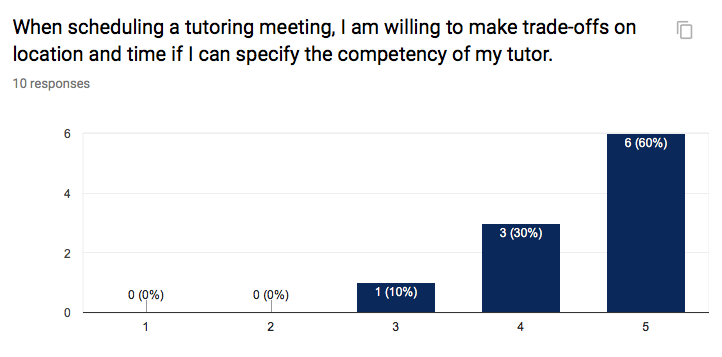
\includegraphics[width=\textwidth]{init_survey_competency}
    % \caption{Average Levels for Frustration, Confusion, and Gaming the System per Student across their entire usage of the Tutoring System}
    \label{fig:scatterplot}
\end{figure*}



\label{sec:possible-enhancements} 

\subsubsection{Enhancements} 
The original creators of WolfTutor proposed
three additional features for future development. The first was to
integrate an online platform to conduct tutoring sessions online. The
second was to allow both the tutor and the student to sync their
session reservation with their calendar, e.g. Google Calendar. Lastly,
to update the scheduling algorithm such that a user could edit or
delete reservations in addition to being able to create and view
them. Our team provided two other features: increasing matching
options between tutors and students and allowing students to browse
their reservation history.

After careful consideration, three main pain points were decided upon
that consisted of the proposed enhancements. Integration of an online
platform was discarded because it was not thought to facilitate the
quality of the match between tutor and student.

\paragraph{Scheduling and Calendar Sync} WolfTutor currently only
allows users seeking a tutoring session to create and view
reservations. In real life, people change their mind or events come up
such that a schedule change is in order. The ability to cancel or
reschedule reservations would make WolfTutor more applicable to real
world scheduling scenarios. In addition, facilitating intergration
with commonly used calendars such as Google and IOS Calendar extends
this principle of making scheduling easier.

\paragraph{Increasing Matching Options} In regards to matching with
tutors, WolfTutor currently displays a list of tutor's and their
ratings based on the student's desired subject. Then, the student may
attempt to book a reservation with a tutor they choose. By expanding
matching options, a student should be able easily find a higher
quality match with a tutor. For example, a student could filter tutors
by location by selecting only locations they want to meet up at in a
checkbox. Similarily, if a student has a few tutors they prefer, they
could select those names from a checkbox such that WolfTutor only
displays those tutors. This type of filtering system is often used by
medical facilities with multiple practioners and multiple practing
sites. It is also used by NC State University's scheduling tool on
epack.

\paragraph{History and Recommendations} WolfTutor does currently allow
for student's to review and rate the tutors that they met with
previously. However, there is no way to view a student's reservation
history past the most recent tutor. WolfTutor also does not provide a
way for a student to easily re-book a new reserveration with a tutor
they chose previously if they liked the tutor and would like to
schedule a reservation with them again. Adding these enhancements
would increase ease of use by helping a student distinguish between a
competent and non-competent tutor they've had in the past.

\begin{figure*}[t]
  \centering
    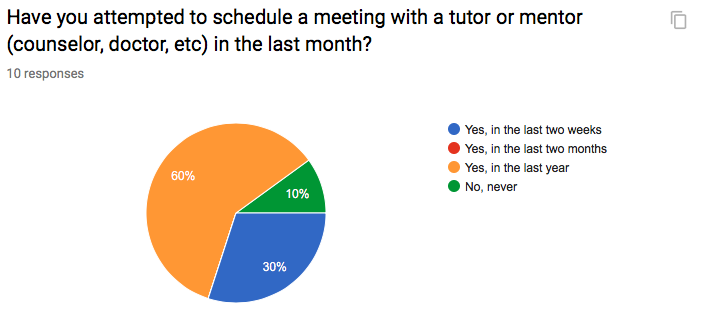
\includegraphics[width=\textwidth]{init_survey_haveyou}
    % \caption{Average Levels for Frustration, Confusion, and Gaming the System per Student across their entire usage of the Tutoring System}
    \label{fig:scatterplot}
\end{figure*}

\subsubsection{Initial Survey}
\label{sec:initial-survey} A survey was conducted to determine which
enhancement the intended user base (students) prefered the most. The
survey was separated into three parts.

\paragraph{Background} A background section measured how prevalent
scheduling was within the daily life of the participants. Most
participants admitted having to schedule a meeting within the last
year.

\paragraph{Priorities} The next section revealed which enhancement the
participants thought was a priority by asking them to rate the level
of important the enhancement was on a scale from 1 (least important)
to 5 (most important). To avoid bias, instead of explaining the
enhancements out, the survey questions were created around the base
point of the enhancement:
\begin{itemize}
  \item "When scheduling a tutoring meeting, picking the location is
very important to me."
  \item "When scheduling a tutoring meeting, the competency of the
tutor is very important to me."
  \item "When scheduling a tutoring meeting, being able to agree on a
time quickly and easily is very important to me."
\end{itemize} The question regarding competency scored the highest
level of important among the participants collectively. Scheduling and
increased matching (by location) followed respectively.

\paragraph{Trade Offs} The objective of the third section was to
validiate the results in the second section by asking the participants
which enhancements they would be willing to compromise on in order to
get the enhancement they thought was more important. The questions
included:
\begin{itemize}
  \item "When scheduling a tutoring meeting, I am willing to make
trade-offs on the competency of the tutor and time if I can specify
the location of the meeting."
  \item "When scheduling a tutoring meeting, I am willing to make
trade-offs on location and time if I can specify the competency of my
tutor."
  \item "When scheduling a tutoring meeting, I am willing to make
trade-offs in location and competency if I can specify the time of the
meeting."
\end{itemize} Again, competency scored the highest as the most
important enhancement collectively. Scheduling followed in second
place and location matching in third.

\paragraph{Other} An option was given to participants to suggest a new
enhancement. The only received response was to integrate the
application with Skype.

\begin{figure*}[ht]
  \centering
    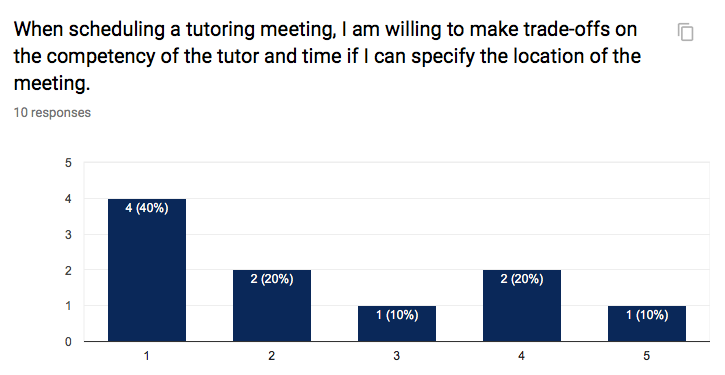
\includegraphics[width=.45\textwidth]{init_survey_location}
    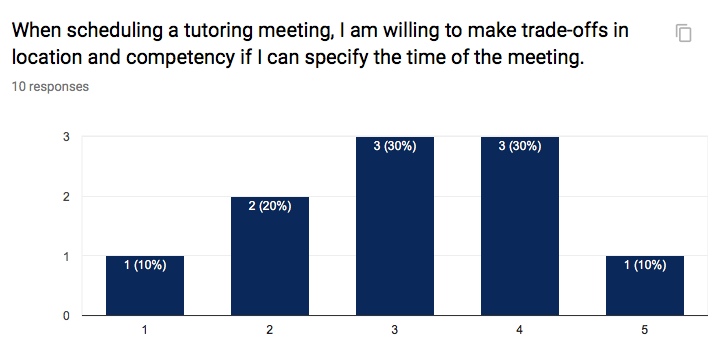
\includegraphics[width=.45\textwidth]{init_survey_time}
\end{figure*}

\subsubsection{Chosen Enhancement}
Since the vast majority of surveyed users from our target audience 
elected easier matching with competent tutors, our chosen enhancement
focuses on tutor matching with regards to the qualities of the tutor that 
make the tutor a good tutor. This enhancement is explained in more detail within section \ref{sec:tutor-matching}.

%%% Local Variables:
%%% mode: latex
%%% TeX-master: "../main"
%%% End:
